\section{Casos de Uso}
\begin{figure}[h]
  \begin{center}
    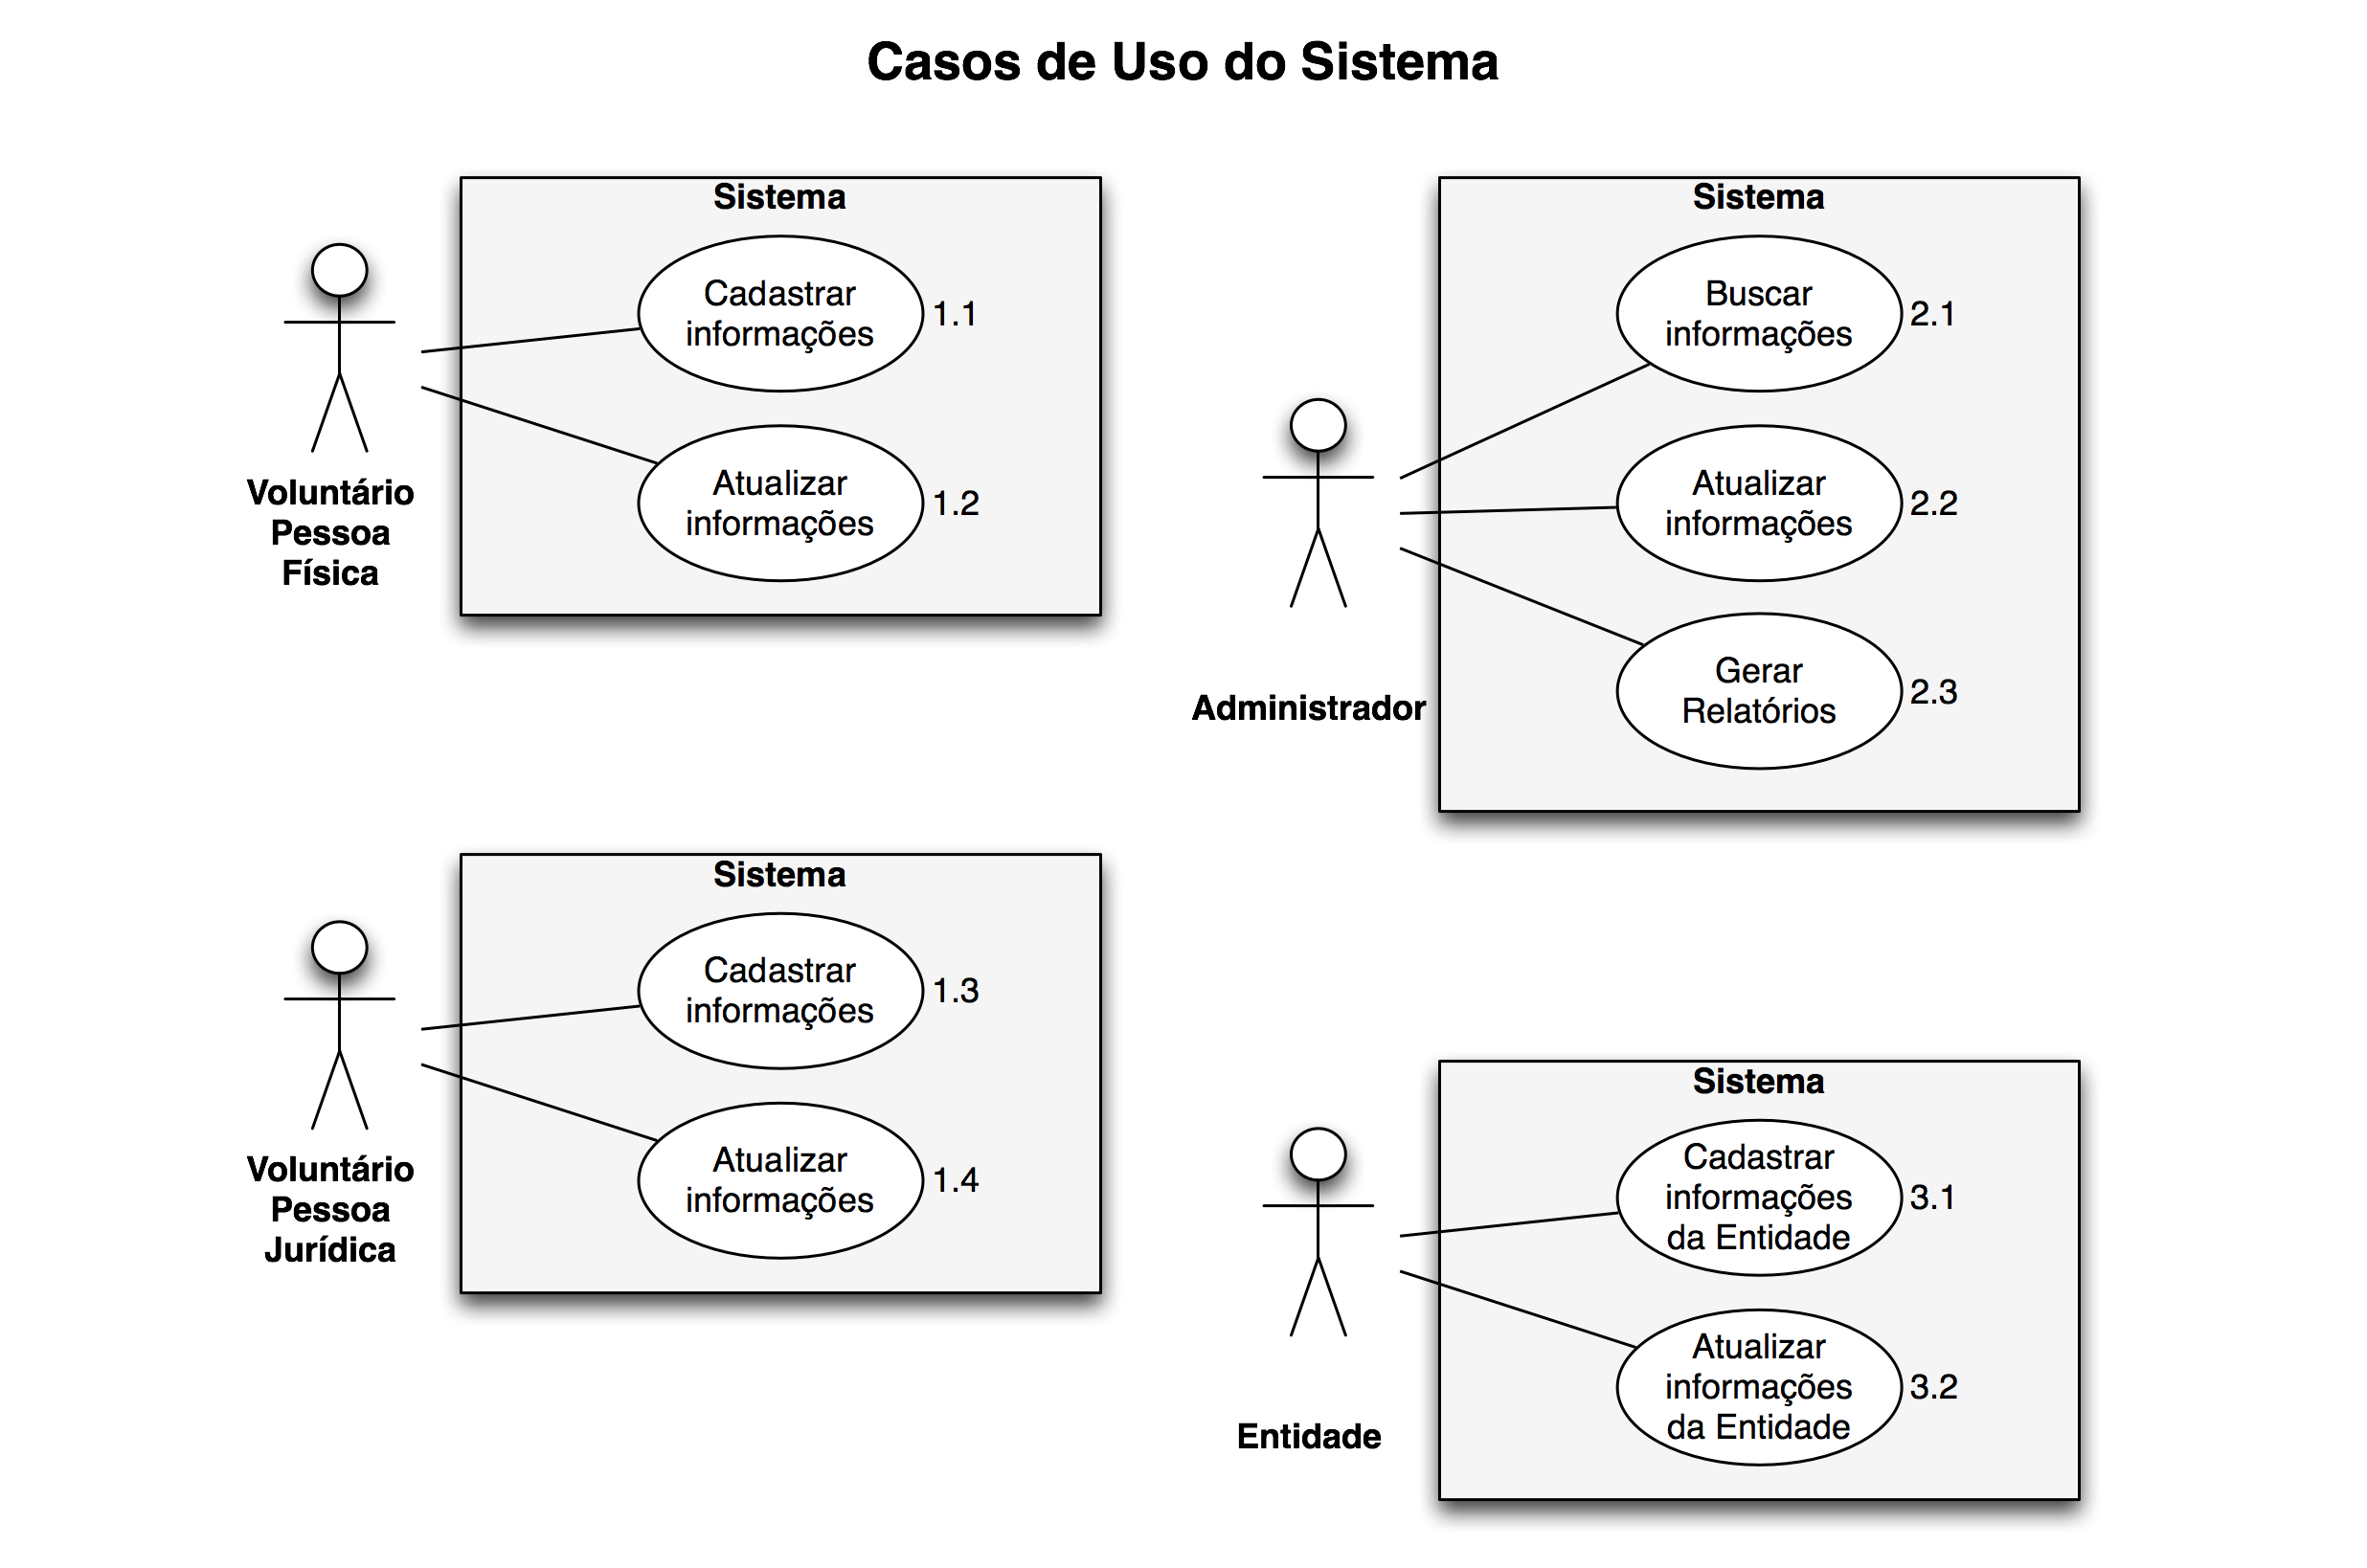
\includegraphics[scale=.6]{casosDeUsoJCI.png}
   \end{center}    
\end{figure}

\newpage
\section{Descrição dos Casos de Uso}
  \subsection{Caso de Uso 1.1}
    \begin{table}[h]
    \begin{center}
    \begin{tabular}{|p{5cm}|p{10cm}|}
      \hline
      Número do caso de uso & 1.1\\
      \hline
      Nome do caso de uso & Cadastrar dados de pessoa físicas.\\
      \hline
      Ator principal & Voluntário (pessoa física).\\
      \hline
      Resumo & Este caso de uso descreve o cadastramento de um voluntário que é uma pessoa física.\\
      \hline
      Pré-Condição & Deve possuir CPF, email e telefone. Dados válidos\\
%      \hline
%      Caso secundário & Insucesso da operação de cadastramento das informações da pessoa física.\\
      \hline
      Fluxo Principal & \\
      \hline
      Ações do ator & Ações do sistema\\
      \hline
      1. O voluntário acessa o site & \\
      \hline   
      2. Clica no link para cadastro & \\
      \hline
      3. O voluntário digita seus dados & \\
      \hline
      4. Clica no link para envio de dados & \\
      \hline
      & 5. Recebe os dados e armazena no banco de dados.\\
      \hline
      Fluxo Alternativo & \\
      \hline
      Ações do ator & Ações do sistema\\
      \hline
      1. O voluntário acessa o site & \\
      \hline   
      2. Clica no link para cadastro & \\
      \hline
      3. O voluntário digita dados inconsistentes & \\
      \hline
      4. Clica no link para envio de dados & \\
      \hline
      & 5. Retorna mensagem de erro \\
      \hline
    \end{tabular}
    \end{center}
    \end{table}
%    \subsubsection{Diagrama de Atividade 1.1}
%    \begin{figure}[H]
%    \begin{center}
%      \includegraphics[scale=.175]{atv1-1.png}
%    \end{center}    
%    \end{figure}
\newpage

  \subsection{Caso de Uso 1.2}
    \begin{table}[h]
    \begin{center}
    \begin{tabular}{|p{5cm}|p{10cm}|}
      \hline
      Número do caso de uso & 1.2\\
      \hline
      Nome do caso de uso & Atualizar informações do voluntário (pessoa física)\\
      \hline
      Ator Principal & Voluntário pessoa física\\
      \hline
      Resumo & Este caso de uso descreve a atualização de dados feita pelo voluntário\\
      \hline
      Pré-Condição & Deve ter sido cadastrado e dados devem ser válidos\\
%      \hline
%      Caso secundário & Insucesso da operação de atualização das informações da pessoa física\\
      \hline
      Fluxo Principal & \\
      \hline
      Ações do ator & Ações do sistema \\
      \hline
      1. O voluntário acessa o site & \\
      \hline
      2. Insere dados de login & \\
      \hline
       & 3. Autentica os dados\\
      \hline
      4. Redigita dados & \\
      \hline
      & 5. Recebe os dados, atualiza e armazena no banco de dados\\
      \hline
      Fluxo Alternativo & \\
      \hline
      Ações do ator & Ações do sistema\\
      \hline
      1. O voluntário acessa o site & \\
      \hline
      2. Insere dados de login & \\
      \hline
       & 3. Autentica os dados\\
      \hline
      4. Redigita dados, mas de forma inconsistente & \\
      \hline
      & 5. Retorna mensagem de erro\\
      \hline
    \end{tabular}
    \end{center}
    \end{table}

%    \subsubsection{Diagrama de Atividade 1.2}
%    \begin{figure}[H]
%    \begin{center}
%      \includegraphics[scale=.175]{atv1-2.png}
%    \end{center}    
%    \end{figure}



\newpage

  \subsection{Caso de Uso 1.3}
    \begin{table}[h]
    \begin{center}
    \begin{tabular}{|p{5cm}|p{10cm}|}
      \hline
      Número do caso de uso & 1.3\\
      \hline
      Nome do caso de uso   & Cadastrar informações pessoa jurídica\\
      \hline
      Ator principal        & Voluntário pessoa jurídica\\
      \hline
      Resumo                & Este caso de uso descreve o cadastramento de um voluntário que é uma pessoa jurídica\\
%      \hline
%      Caso secundário       & Insucesso da operação de cadastramento das informações da pessoa jurídica\\
      \hline
      Pré-Condicão          & Deve possuir CNPJ, email e telefone\\
      \hline
      Fluxo Principal       & \\
      \hline
      Ações do ator         & Ações do sistema\\
      \hline
      1. O voluntário acessa o site & \\
      \hline
      2. Clica no link para cadastro & \\
      \hline
      3. O voluntário digita seus dados & \\
      \hline
      4. Clica no link para envio de dados & \\
      \hline
      & 5. Recebe os dados e armazena no banco de dados\\
      \hline
      Fluxo Alternativo & \\
      \hline
      Ações do ator & Ações do sistema\\
      \hline
      1. O voluntário acessa o site & \\
      \hline
      2. Insere dados de login & \\
      \hline
       & 3. Autentica os dados\\
      \hline
      4. Redigita dados, mas de forma inconsistente & \\
      \hline
      & 5. Retorna mensagem de erro\\
      \hline
    \end{tabular}
    \end{center}
    \end{table}

%    \subsubsection{Diagrama de Atividade 1.3}
%    \begin{figure}[H]
%    \begin{center}
%      \includegraphics[scale=.175]{atv1-3.png}
%    \end{center}    
%    \end{figure}



\newpage

  \subsection{Caso de Uso 1.4}
    \begin{table}[h]
    \begin{center}
    \begin{tabular}{|p{5cm}|p{10cm}|}
      \hline
      Número do caso de uso & 1.4\\
      \hline
      Nome do caso de uso   & Atualizar informações do voluntário pessoa jurídica\\
      \hline
      Ator principal        & Voluntário pessoa jurídica\\
      \hline
      Resumo                & Este caso de uso descreve a atualização de dados feita pelo voluntário\\
%      \hline
%      Caso secundário       & Insucesso da operação de atualizações da pessoa jurídica\\
      \hline
      Pré-Condicão          & Deve ter dados cadastrados e dados válidos\\
      \hline
      Fluxo Principal       & \\
      \hline
      Ações do ator         & Ações do sistema \\
      \hline
      1. O voluntário acessa ao site & \\
      \hline
      2. Insere dados de login & \\
      \hline
      & 3. Autentica os dados\\
      \hline
      4. Reedita seus dados & \\
      \hline
      & 5. Recebe os dados, atualiza e armazena no banco de dados\\
      \hline
      Fluxo Alternativo & \\
      \hline
      Ações do ator & Ações do sistema\\
      \hline
      1. O voluntário acessa o site & \\
      \hline
      2. Insere dados de login & \\
      \hline
       & 3. Autentica os dados\\
      \hline
      4. Redigita dados, mas de forma inconsistente & \\
      \hline
      & 5. Retorna mensagem de erro\\
      \hline
    \end{tabular}
    \end{center}
    \end{table}

%    \subsubsection{Diagrama de Atividade 1.4}
%    \begin{figure}[H]
%    \begin{center}
%      \includegraphics[scale=.175]{atv1-4.png}
%    \end{center}    
%    \end{figure}


\newpage

  \subsection{Caso de Uso 2.1}
    \begin{table}[h]
    \begin{center}
    \begin{tabular}{|p{5cm}|p{10cm}|}
      \hline
      Número do caso de uso & 2.1\\ 
      \hline
      Nome do caso de uso   & Acesso às informações cadastradas\\
      \hline
      Ator principal        & Administrador\\
      \hline
      Resumo                & Este caso de uso descreve o acesso do Administrador aos dados cadastrados\\
      \hline
      Fluxo Principal       & \\
      \hline
      Ações do ator         & Ações do sistema \\
      \hline
      1. Solicita informações sobre os voluntários & \\
      \hline
      & 2. Fornece as informações requisitadas\\
      \hline
      3. Obtém informações & \\
      \hline

      
    \end{tabular}
    \end{center}
    \end{table}

%    \subsubsection{Diagrama de Atividade 2.1}
%    \begin{figure}[H]
%    \begin{center}
%      \includegraphics[scale=.175]{atv2-1.png}
%    \end{center}    
%    \end{figure}


\newpage

  \subsection{Caso de Uso 2.2}
    \begin{table}[h]
    \begin{center}
    \begin{tabular}{|p{5cm}|p{10cm}|}
      \hline
      Número do caso de uso & 2.2\\
      \hline
      Nome do caso de uso   & Atualizar dados cadastrados\\
      \hline
      Ator principal        & Administrador\\
      \hline
      Resumo                & Este caso de uso descreve a atualização dos dados feita pelo administrador\\
      \hline
      Fluxo Principal       & \\
      \hline
      Ações do ator         & Ações do sistema \\
      \hline
      1. Solicitar informações & \\
      \hline
      & 2. Fornece informações \\
      \hline
      3. Obtém informações & \\
      \hline
      4. Redigita informações & \\
      \hline
      & 5. Atualiza e armazena no banco de dados\\
      \hline
      Fluxo Alternativo & \\
      \hline
      Ações do ator & Ações do sistema\\
      \hline
      1. Solicitar informações & \\
      \hline
      & 2. Fornece informações \\
      \hline
      3. Obtém informações & \\
      \hline
      4. Redigita informações, mas de forma inconsistente & \\
      \hline
      & 5. Retorna mensagem de erro\\
      \hline      
    \end{tabular}
    \end{center}
    \end{table}

%    \subsubsection{Diagrama de Atividade 2.2}
%    \begin{figure}[H]
%    \begin{center}
%      \includegraphics[scale=.175]{atv2-2.png}
%    \end{center}    
%    \end{figure}


\newpage

  \subsection{Caso de Uso 2.3}
    \begin{table}[h]
    \begin{center}
      \begin{tabular}{|p{5cm}|p{10cm}|}
      \hline
      Número do caso de uso & 2.3\\
      \hline
      Nome do caso de uso   & Gerar relátorio de entidades ou voluntários\\
      \hline
      Ator principal        & Administrador\\
      \hline
      Resumo                & Este caso de uso descreve o acesso do administrador as informações cadastradas pelos voluntários ou entidades para gerar um relatório.\\
      \hline
      Fluxo Principal       & \\
      \hline
      Ações do ator         & Ações do sistema \\
      \hline
      1. Solicitar informações sobre os voluntários ou entidades, através de um conjunto de características & \\ 
      \hline
      & 2. Fornece a lista de voluntários ou entidades conforme informações requisitadas\\
      \hline
      3. Obtém informações & \\
      \hline
      4. Clica para gerar relátorio & \\
      \hline
      & 5. Gera o relatório\\
      \hline
      
    \end{tabular}
    \end{center}
    \end{table}

%    \subsubsection{Diagrama de Atividade 2.3}
%    \begin{figure}[H]
%    \begin{center}
%      \includegraphics[scale=.175]{atv2-3.png}
%    \end{center}    
%    \end{figure}


\newpage

  \subsection{Caso de Uso 3.1}
    \begin{table}[h]
    \begin{center}
    \begin{tabular}{|p{5cm}|p{10cm}|}
      \hline
      Número do caso de uso & 3.1\\
      \hline
      Nome do caso de uso & Cadastrar informações da entidade\\
      \hline
      Ator principal & Entidade\\
      \hline
      Resumo & Este caso de uso descreve o cadastramento de uma entidade\\
      \hline
      Pré-Condição & Deve possuir CNPJ e telefone\\
%      \hline
%      Caso secundário & Insucesso da operação de cadastramento das informações da entidade\\
      \hline
      Fluxo Principal \\
      \hline
      Ações do ator & Ações do sistema\\
      \hline
      1. A entidade acessa o site & \\
      \hline   
      2. Clica no link para cadastro & \\
      \hline
      3. A entidade digita seus dados & \\
      \hline
      4. Clica no link para envio de dados & \\
      \hline
      & 5. Recebe os dados e armazena no banco de dados.\\
      \hline
      Fluxo Principal       & \\
      \hline
      Ações do ator         & Ações do sistema \\
      \hline
      1. A entidade acessa o site & \\
      \hline   
      2. Clica no link para cadastro & \\
      \hline
      3. A entidade digita seus dados, mas de forma inconsistente & \\
      \hline
      4. Clica no link para envio de dados & \\
      \hline
      & 5. Retorna mensagem de erro\\
      \hline
    \end{tabular}
    \end{center}
    \end{table}
%    \subsubsection{Diagrama de Atividade 3.1}
%    \begin{figure}[H]
%    \begin{center}
%      \includegraphics[scale=.175]{atv3-1.png}
%    \end{center}    
%    \end{figure}
\newpage

  \subsection{Caso de Uso 3.2}
    \begin{table}[h]
    \begin{center}
    \begin{tabular}{|p{5cm}|p{10cm}|}
      \hline
      Número do caso de uso & 1.2\\
      \hline
      Nome do caso de uso & Atualizar informações da entidade\\
      \hline
      Ator Principal & Entidade\\
      \hline
      Resumo & Este caso de uso descreve a atualização de dados feita pela entidade\\
      \hline
      Pré-Condição & Deve ter sido cadastrado e dados devem ser válidos\\
%      \hline
%      Caso secundário & Insucesso da operação de atualização das informações da entidade\\
      \hline
      Fluxo Principal & \\
      \hline
      Ações do ator & Ações do sistema \\
      \hline
      1. A entidade acessa o site & \\
      \hline
      2. Insere dados de login & \\
      \hline
       & 3. Autentica os dados\\
      \hline
      4. Redigita dados & \\
      \hline
      & 5. Recebe os dados, atualiza e armazena no banco de dados\\
      \hline
      Fluxo Principal       & \\
      \hline
      Ações do ator         & Ações do sistema \\
      \hline
      1. A entidade acessa o site & \\
      \hline
      2. Insere dados de login & \\
      \hline
       & 3. Autentica os dados\\
      \hline
      4. Redigita dados, mas de forma inconsistente & \\
      \hline
      & 5. Retorna mensagem de erro\\
      \hline
    \end{tabular}
    \end{center}
    \end{table}

%    \subsubsection{Diagrama de Atividade 3.2}
%    \begin{figure}[H]
%    \begin{center}
%      \includegraphics[scale=.175]{atv3-2.png}
%    \end{center}    
%    \end{figure}

% \subsection{Caso de Uso 1.2}
%   \begin{table}[h]
%   \begin{center}
%   \begin{tabular}{p{5cm}|p{10cm}}
%      Número do caso de uso & 
%     \hline
%     Nome do caso de uso   & 
%     \hline
%     Ator principal        & 
%     \hline
%     Resumo                & 
%     \hline
%     Caso secundário       & 
%     \hline
%     Pré-Condicão          & 
%     \hline
%     Fluxo Principal       & 
%     \hline
%     Ações do ator         & Ações do sistema \\
%     \hline
%
%    
%  \end{tabular}
%  \end{center}
%  \end{table}
%
%  \subsubsection{Diagrama de Atividade 1.2}
%  \begin{figure}[H]
%  \begin{center}
%    \includegraphics[scale=.175]{atv1-2.png}
%  \end{center}    
%  \end{figure}

